\documentclass[a4paper,11pt]{article}

\usepackage{amsmath}
\usepackage[pdftex]{graphicx}

\usepackage[english,greek]{babel}

\usepackage{lmodern}

\usepackage{listings}

\lstset{
  basicstyle=\ttfamily,
  columns=fullflexible,
  frame=single,
  breaklines=true
}

% Αφαίρεσε (Εισήγαγε) την παρακάτω γραμμή σε σχόλιο αν ο επεξεργαστής κειμένου (δεν) χρησιμοποιεί κωδικοποίηση Unicode για Ελληνικά
\usepackage[utf8x]{inputenc}

% Αφαίρεσε (Εισήγαγε) την παρακάτω γραμμή σε σχόλιο αν ο επεξεργαστής κειμένου (δεν) χρησιμοποιεί κωδικοποίηση iso-8859-7 για Ελληνικά
%\usepackage[iso-8859-7]{inputenc}

%Δημιουργία συντομεύσεων για αλλαγή γραφής σε Ελληνικά/Αγγλικά
\newcommand{\lt}{\latintext}
\newcommand{\gt}{\greektext}

\title{2η Υποχρεωτική Εργασία \\ Στο Μάθημα της Αριθμητικής Ανάλυσης: \\ Άσκηση 6}
\author{Ονοματεπώνυμο: Μπαρακλιλής Ιωάννης  \\  ΑΕΜ: 3685}
\date{12 Ιανουαρίου 2021}

\begin{document}

\maketitle
\section{Επιλογή σημείων}
Ζητείται ο υπολογισμός του ολοκληρώματος του ημίτονου με τις μεθόδους {\lt Simpson} και τραπεζίου στο διάστημα $[0, \dfrac{\pi}{2}]$ με επιλογή 11 σημείων.\\
Οι μέθοδοι αυτές απαιτούν τον διαχωρισμό του επιλεγμένου διαστήματος ολοκλήρωσης σε έναν (άρτιο) αριθμό (έστω Ν) από ισομήκη διαστήματα. Εφόσον ζητούνται 11 σημεία, θα χωρίσω το διάστημα $[0, \dfrac{\pi}{2}]$ σε 10 ισομήκη διαστήματα των οποίων τα σημεία {\lt $x_i$} επιλέγονται χρησιμοποιώντας τον τύπο {\lt $x_i = x_0 + k\dfrac{b-a}{N}, k = 0,...,N$} με πρώτο σημείο το αρχικό σημείο ολοκλήρωσης {\lt $a = 0$} και τελικό σημείο το σημείο {\lt $b = \dfrac{\pi}{2}$}. Επομένως έχω τα σημεία {\lt $x_i = x_0 + k\dfrac{b-a}{N} = k\dfrac{\pi}{20}$}.\\
Αναλυτικά, έχω τα σημεία:
\lt
\begin{enumerate}
    \item $x_0 = a = 0$
    \item $x_1 = \dfrac{\pi}{20}$
    \item $x_2 = \dfrac{\pi}{10}$
    \item $x_3 = \dfrac{3\pi}{20}$
    \item $x_4 = \dfrac{\pi}{5}$
    \item $x_5 = \dfrac{\pi}{4}$
    \item $x_6 = \dfrac{3\pi}{10}$
    \item $x_7 = \dfrac{7\pi}{20}$
    \item $x_8 = \dfrac{2\pi}{5}$
    \item $x_9 = \dfrac{9\pi}{20}$
    \item $x_{10} = b = \dfrac{\pi}{2}$
\end{enumerate}
\gt
τα οποία απέχουν μεταξύ τους {\lt $\dfrac{\pi}{20}$}

\section{Υπολογισμός ολοκληρώματος ημιτόνου με μέθοδο {\lt Simpson}}
Το ζητούμενο υλοποιείται προγραμματιστικά στην γλώσσα {\lt python} (3.7) στο αρχείο {\lt a\textunderscore simpson\textunderscore integration.py} το οποίο φαίνεται παρακάτω:\\

\lt
\lstinputlisting[language=Python]{a_simpson_integration.py}
\gt

\par
Στον παραπάνω κώδικα:\\
\par
Αρχικά, εισάγονται (γίνονται {\lt import}) η συνάρτηση {\lt sin} και σταθερά {\lt pi} από την βιβλιοθήκη {\lt math} που θα χρειαστούν στην συνέχεια.\\
\par
Στην συνέχεια ορίζεται η συνάρτηση {\lt simpson\textunderscore integral\textunderscore from\textunderscore points} η οποία δέχεται έναν δισδιάστατο πίνακα στον οποίο κάθε γραμμή αναπαριστά ένα ζεύγος σημείων {\lt $(x, y = f(x))$} ({\lt f} η συνάρτηση που ολοκληρώνεται) όπου η πρώτη στήλη περιέχει τα επιλεγμένα σημεία {\lt $x$} τα οποία θα χρησιμοποιηθούν από την μέθοδο {\lt Simpson} και η δεύτερη στήλη την τιμή της συνάρτησης στο αντίστοιχο σημείο (θεωρείται δεδομένο ότι τα σημεία αυτά αποτελούν ομοιόμορφο διαμερισμό του {\lt $[a, b]$} και  ότι $x_0 < x_1 < ... < x_N$) και επιστρέφει το ολοκλήρωμα της συνάρτησης συνάρτησης (των δοθέντων σημείων) στο διάστημα {\lt $[a, b]$} όπου {\lt a} είναι το πρώτο και {\lt b} το τελευταίο {\lt x} των δοθέντων σημείων.\\
Αναλυτικά:\\
Αρχικά, ορίζω και αρχικοποιώ σε 0 την μεταβλητή {\lt func\textunderscore sum} η οποία θα αποθηκεύει το άθροισμα των τιμών της {\lt f} σύμφωνα με τον τύπο {\lt $f(x_0) + f(x_N) + 2\sum_{i=1}^{\frac{N}{2}-1}f(x_{2i}) + 4\sum_{i=1}^{\frac{N}{2}}f(x_{2i-1})$} της θεωρίας.\\
Στην συνέχεια, ορίζω τις μεταβλητές {\lt a, b, N} (για ευκολία κατανόησης αντιστοίχησης μαθηματικών τύπων στον αλγόριθμο) που αποθηκεύουν το αρχικό και τελικό σημείο του διαστήματος και τον αριθμό ισομηκών διαστημάτων, αντίστοιχα.\\
Ακολούθως, (χρησιμοποιώντας την μεταβλητή {\lt temp\textunderscore sum} που αποθηκεύει τα ενδιάμεσα αθροίσματα) υπολογίζω και αποθηκεύω στην μεταβλητή {\lt func\textunderscore sum} την τιμή {\lt $f(x_0) + f(x_N) + 2\sum_{i=1}^{\frac{N}{2}-1}f(x_{2i}) + 4\sum_{i=1}^{\frac{N}{2}}f(x_{2i-1})$} χρησιμοποιώντας τα δοθέντα σημεία της παραμέτρου.\\
Τέλος, υπολογίζω και επιστρέφω την τελική τιμή (που αποτελεί προσέγγιση του ολοκληρώματος) σύμφωνα με τον τύπο {\lt $\dfrac{b-a}{3N}(f(x_0) + f(x_N) + 2\sum_{i=1}^{\frac{N}{2}-1}f(x_{2i}) + 4\sum_{i=1}^{\frac{N}{2}}f(x_{2i-1}))$}, της θεωρίας.\\

\par
Μετά, ορίζεται η συνάρτηση {\lt main} που δεν δέχεται ορίσματα και εκτελείται άμεσα όταν εκτελέσουμε το παραπάνω αρχείο που εκτελεί και εμφανίζει στην οθόνη τους ζητούμενους υπολογισμούς χρησιμοποιώντας την παραπάνω μέθοδο και τα σημεία που ορίστηκαν στο πρώτο μέρος της αναφοράς.\\
Αναλυτικά:\\
Αρχικά, ορίζονται τα παραπάνω (του πρώτου μέρους της αναφοράς) σημεία στον πίνακα {\lt chosen\textunderscore points} (χρησιμοποιώντας τα σημεία που επιλέχθηκαν προηγουμένως και το ημίτονο που αντιστοιχεί σε κάθε ένα που υπολογίζουμε με την συνάρτηση {\lt sin} της βιβλιοθήκης {\lt math}) μετά ορίζονται {\lt a, b, N} (για ευκολία κατανόησης αντιστοίχησης μαθηματικών τύπων στον αλγόριθμο) που αποθηκεύουν το αρχικό και τελικό σημείο του διαστήματος και τον αριθμό ισομηκών διαστημάτων, αντίστοιχα.\\
Μετά, υπολογίζονται και εμφανίζονται:
\begin{enumerate}
    \item Το ολοκλήρωμα του ημιτόνου στο διάστημα $[0, \frac{\pi}{2}]$ χρησιμοποιώντας την συνάρτηση {\lt simpson\textunderscore integral\textunderscore from\textunderscore points} και τον πίνακα {\lt chosen\textunderscore points} που ορίστηκαν προηγουμένως.
    \item Το μέγιστο θεωρητικό σφάλμα του υπολογισμού ολοκληρώματος με την μέθοδο {\lt Simpson} χρησιμοποιώντας τον τύπο {\lt $\lvert e\rvert \leq \dfrac{(b-a)^5}{180N^4}M = \dfrac{(b-a)^5}{180N^4}$} γιατί, {\lt $M = \max\{ \lvert f^{(4)}(x)\rvert : x \in [a, b] = [0, \dfrac{\pi}{2}]\} \Longrightarrow M = 1$} εφόσον {\lt $(sin(x))^{(4)} = sin(x)$} και {\lt $\max\{ \lvert sin(x)\rvert : x \in [0, \dfrac{\pi}{2}]\} = 1$ }
    \item Το αριθμητικό σφάλμα αφαιρώντας από το ολοκλήρωμα που υπολογίστηκε προηγουμένως την τιμή (με άπειρη ακρίβεια) του ολοκληρώματος {\lt $\int_{0}^{\frac{\pi}{2}}sin(x)dx = 1$}.
\end{enumerate}

\par
Αν εκτελέσουμε το παραπάνω αρχείο θα έχουμε ως αποτέλεσμα (στην οθόνη) το ακόλουθο:\\
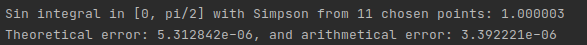
\includegraphics[width=\linewidth]{Exercise6/run_a.png}\\

Επομένως, τα αποτελέσματα είναι τα ακόλουθα:
\begin{itemize}
    \item Ολοκλήρωμα με μέθοδο {\lt Simpson} στο διάστημα $[0, \frac{\pi}{2}]$ (με υποδιαστήματα που ορίζονται από τα παραπάνω σημεία) το 1.000003,
    \item (Μέγιστο) Θεωρητικό σφάλμα το $\simeq 0.531\cdot 10^{-7}$ και
    \item Αριθμητικό σφάλμα το $\simeq 0.392\cdot 10^{-6}$
\end{itemize}

\section{Υπολογισμός ολοκληρώματος ημιτόνου με μέθοδο τραπεζίου}
Το ζητούμενο υλοποιείται προγραμματιστικά στην γλώσσα {\lt python} (3.7) στο αρχείο {\lt b\textunderscore trapezoid\textunderscore integration.py} το οποίο φαίνεται παρακάτω:\\

\lt
\lstinputlisting[language=Python]{b_trapezoid_integration.py}
\gt

\par
Στον παραπάνω κώδικα:\\
\par
Αρχικά, εισάγονται (γίνονται {\lt import}) η συνάρτηση {\lt sin} και σταθερά {\lt pi} από την βιβλιοθήκη {\lt math} που θα χρειαστούν στην συνέχεια.\\
\par
Στην συνέχεια ορίζεται η συνάρτηση {\lt trapezoid\textunderscore integral\textunderscore from\textunderscore points} η οποία δέχεται έναν δισδιάστατο πίνακα στον οποίο κάθε γραμμή αναπαριστά ένα ζεύγος σημείων {\lt $(x, y = f(x))$} ({\lt f} η συνάρτηση που ολοκληρώνεται) όπου η πρώτη στήλη περιέχει τα επιλεγμένα σημεία {\lt $x$} τα οποία θα χρησιμοποιηθούν από την μέθοδο τραπεζίου και η δεύτερη στήλη την τιμή της συνάρτησης στο αντίστοιχο σημείο (θεωρείται δεδομένο ότι τα σημεία αυτά αποτελούν ομοιόμορφο διαμερισμό του {\lt $[a, b]$} και  ότι $x_0 < x_1 < ... < x_N$) και επιστρέφει το ολοκλήρωμα της συνάρτησης συνάρτησης (των δοθέντων σημείων) στο διάστημα {\lt $[a, b]$} όπου {\lt a} είναι το πρώτο και {\lt b} το τελευταίο {\lt x} των δοθέντων σημείων.\\
Αναλυτικά:\\
Αρχικά, ορίζω και αρχικοποιώ σε 0 την μεταβλητή {\lt func\textunderscore sum} η οποία θα αποθηκεύει το άθροισμα των τιμών της {\lt f} σύμφωνα με τον τύπο {\lt $f(x_0) + f(x_N) + 2\sum_{i=1}^{N-1}f(x_{i})$} της θεωρίας.\\
Στην συνέχεια, ορίζω τις μεταβλητές {\lt a, b, N} (για ευκολία κατανόησης αντιστοίχησης μαθηματικών τύπων στον αλγόριθμο) που αποθηκεύουν το αρχικό και τελικό σημείο του διαστήματος και τον αριθμό ισομήκη διαστημάτων, αντίστοιχα.\\
Ακολούθως, (χρησιμοποιώντας την μεταβλητή {\lt temp\textunderscore sum} που αποθηκεύει τα ενδιάμεσα αθροίσματα) υπολογίζω και αποθηκεύω στην μεταβλητή {\lt func\textunderscore sum} την τιμή {\lt $f(x_0) + f(x_N) + 2\sum_{i=1}^{N-1}f(x_{i})$} χρησιμοποιώντας τα δοθέντα σημεία της παραμέτρου.\\
Τέλος, υπολογίζω και επιστρέφω την τελική τιμή (που αποτελεί προσέγγιση του ολοκληρώματος) σύμφωνα με τον τύπο {\lt $\dfrac{b-a}{2N}(f(x_0) + f(x_N) + 2\sum_{i=1}^{N-1}f(x_{i}))$} της θεωρίας.\\

\par
Μετά, ορίζεται η συνάρτηση {\lt main} που δεν δέχεται ορίσματα και εκτελείται άμεσα όταν εκτελέσουμε το παραπάνω αρχείο που εκτελεί και εμφανίζει στην οθόνη τους ζητούμενους υπολογισμούς χρησιμοποιώντας την παραπάνω μέθοδο και τα σημεία που ορίστηκαν στο πρώτο μέρος της αναφοράς.\\
Αναλυτικά:\\
Αρχικά, ορίζονται τα παραπάνω (του πρώτου μέρους της αναφοράς) σημεία στον πίνακα {\lt chosen\textunderscore points} (χρησιμοποιώντας τα σημεία που επιλέχθηκαν προηγουμένως και το ημίτονο που αντιστοιχεί σε κάθε ένα που υπολογίζουμε με την συνάρτηση {\lt sin} της βιβλιοθήκης {\lt math}) μετά ορίζονται {\lt a, b, N} (για ευκολία κατανόησης αντιστοίχησης μαθηματικών τύπων στον αλγόριθμο) που αποθηκεύουν το αρχικό και τελικό σημείο του διαστήματος και τον αριθμό ισομηκών διαστημάτων, αντίστοιχα.\\
Μετά, υπολογίζονται και εμφανίζονται:
\begin{enumerate}
    \item Το ολοκλήρωμα του ημιτόνου στο διάστημα $[0, \frac{\pi}{2}]$ χρησιμοποιώντας την συνάρτηση {\lt trapezoid\textunderscore integral\textunderscore from\textunderscore points} και τον πίνακα {\lt chosen\textunderscore points} που ορίστηκαν προηγουμένως.
    \item Το μέγιστο θεωρητικό σφάλμα του υπολογισμού ολοκληρώματος με την μέθοδο τραπεζίου χρησιμοποιώντας τον τύπο {\lt $\lvert e\rvert \leq \dfrac{(b-a)^3}{12N^2}M =\dfrac{(b-a)^3}{12N^2}$} γιατί, {\lt $M = \max\{ \lvert f^{''}(x)\rvert : x \in [a, b] = [0,\dfrac{\pi}{2}]\} \Longrightarrow M = 1$} εφόσον {\lt $(sin(x))^{''} = -sin(x)$} και {\lt $\max\{ \lvert -sin(x)\rvert : x \in [0,\dfrac{\pi}{2}]\} = 1$ }
    \item Το αριθμητικό σφάλμα αφαιρώντας από το ολοκλήρωμα που υπολογίστηκε προηγουμένως την τιμή (με άπειρη ακρίβεια) του ολοκληρώματος {\lt $\int_{0}^{\frac{\pi}{2}}sin(x)dx = 1$}.
\end{enumerate}

\par
Αν εκτελέσουμε το παραπάνω αρχείο θα έχουμε ως αποτέλεσμα (στην οθόνη) το ακόλουθο:\\
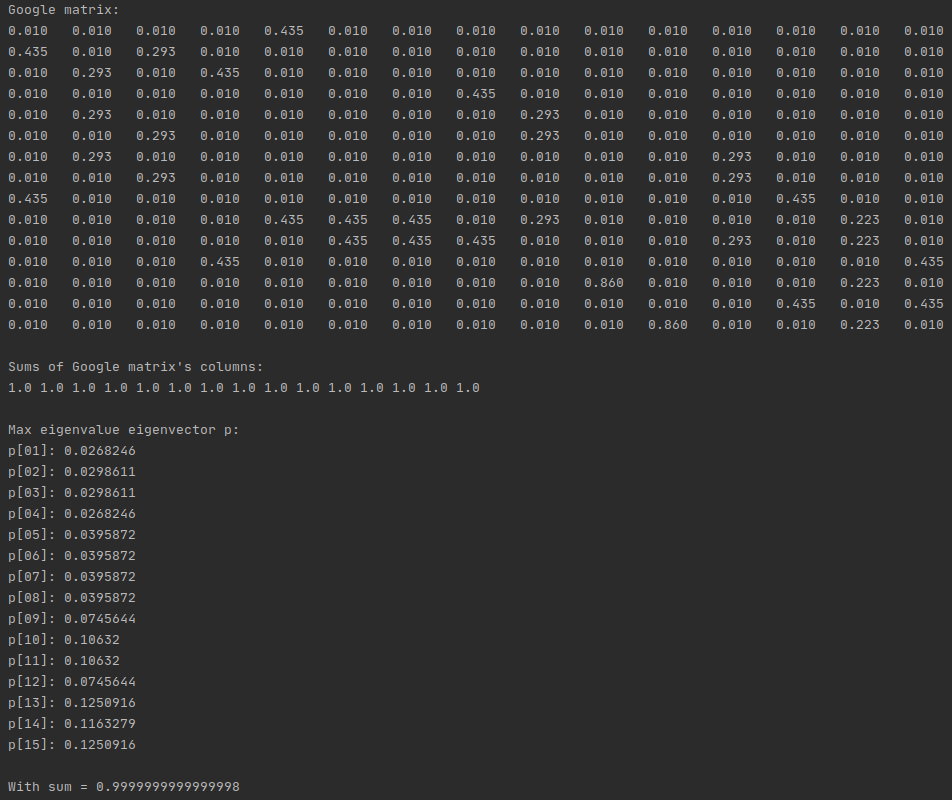
\includegraphics[width=\linewidth]{Exercise6/run_b.png}\\

Επομένως, τα αποτελέσματα είναι τα ακόλουθα:
\begin{itemize}
    \item Ολοκλήρωμα με μέθοδο τραπεζίου στο διάστημα $[0, \frac{\pi}{2}]$ (με υποδιαστήματα που ορίζονται από τα παραπάνω σημεία) το 0.997943,
    \item (Μέγιστο) Θεωρητικό σφάλμα το $\simeq 0.323\cdot 10^{-4}$ και
    \item Αριθμητικό σφάλμα το $\simeq -0.206\cdot 10^{-4}$
\end{itemize}


\end{document}
